\documentclass[num-refs]{wiley-article}
%\documentclass[blind,alpha-refs]{wiley-article}

\usepackage{amsmath,graphicx}
\usepackage{anyfontsize}
\usepackage{siunitx}
\usepackage{silence}
% Links


% Update article type if known
\papertype{Original Article}
% Include section in journal if known, otherwise delete
\paperfield{Journal Section}

\title{ Segmentation of prostate and prostate zones using 3D Convolutional Networks: a multiple MRI vendor analysis }
%\title{ Towards a universal MRI atlas of the prostate and prostate zones. Part II: Deep Learning }

% List abbreviations here, if any. Please note that it is preferred that abbreviations be defined at the first instance they appear in the text, rather than creating an abbreviations list.
\abbrevs{PZ, pheriperal zone; CNN, Convolutional Neural Network; DSC,  S\o rosen-Dice coefficient TZ, transition zone; ROI, region of interest; SGD, Stochastic Gradient Descent}

% Include full author names and degrees, when required by the journal.
% Use the \authfn to add symbols for additional footnotes and present addresses, if any. Usually start with 1 for notes about author contributions; then continuing with 2 etc if any author has a different present address.
\author[1]{Olmo Zavala-Romero PhD}
\author[1]{Adrian L. Breto }
\author[1]{Nicole Gautney}
\author[1]{Yu-Cherng C. Chan}
\author[1]{Alan Dal Pra}
\author[1]{Alan Pollack}
\author[1]{Radka Stoyanova}

\affil[1]{Radiation Oncology, University of Miami Miller School of Medicine,
                Miami, FL, 33136, USA}

\corraddress{Olmo Zavala-Romero PhD, 
            Radiation Oncology, University of Miami Miller School of Medicine,
            Miami, FL, 33136, USA}

\corremail{osz1@med.miami.edu}

\fundinginfo{Funder One, Funder One Department, Grant/Award Number: 123456, 123457 and 123458; 
Funder Two, Funder Two Department, Grant/Award Number: 123459}

\runningauthor{Olmo Zavala-Romero et al.}

\begin{document}
\maketitle

\begin{abstract} % 250 words for all manuscript types
\small{
\textbf{Purpose:} Develop an automatic segmentation algorithm for the prostate and its peripheral zone (PZ) that
is robust across multiple MRI vendors. \\
\textbf{Methods:} A modified version of the 3D U-net neural network is used for automatic segmentation of the prostate and its PZ using multiplanar MRI. The network is a multi-stream convolutional neural network that uses axial, coronal, and sagittal MRI series as input. The preprocessing of the input data includes image normalization, bias correction, and resampling of the images and ground truth contours. A large dataset of 550 scans from multiple MRI vendors (Siemens and GE), is used to test the proposed network. Six different models were trained, three for the prostate and three for the PZ, splitting and combining the training datasets with each MRI vendor. The S\o rosen-Dice coefficient (DSC) is used to compare the performance of the system. \\
\textbf{Results:} The best model achieves DSCs of $0.896 \pm 0.037$ and  $0.830 \pm 0.054$ for segmenting the prostate in each dataset respectively (Siemens and GE). For PZ segmentation, the DSCs of the top model are $0.813 \pm 0.079$ and $0.797 \pm 0.093$. The leading results are consistently obtained when the network is trained with the combined dataset, with just one exception. \\
\textbf{Conclusion:} The proposed system has a performance comparable to the inter-observer variability for segmenting the prostate and its PZ from MRI. Combining images from different MRI vendors on the training of the network is of paramount importance for building a universal model for prostate and PZ segmentation. 
\keywords{ Prostate Zones, Segmentation, MRI, Deep Learning, U-Net}
\end{abstract}

% Paper 5000 words, 10 Figures and tables
% Note 2800 words, 5 Figures and tables
% Other info: 
%   * Figures sub-parts should be labeled a,b,c, etc. 
%   * Figures should not be embedded within the manuscript text 
%   * Figures in Tiff format
%   * Please include all the figure captions, in list format, at the end of your manuscript text file

\section{Introduction}
\label{sec:intro}
Accurate prostate segmentation on MRI datasets is required for many clinical and research 
applications. Furthermore, due to the different imaging properties of the peripheral (PZ) 
and transition zones (TZ) of the prostate, accurate zonal segmentation is also necessary. 
The prostate and zonal contours are necessary for computer aided diagnosis (CAD)
applications for staging, diagnosis, and treatment planning for prostate cancer. In 
a series of applications, prostate contours are fused with ultrasound images to
guide prostate biopsies. Automatic segmentation of the prostate, PZ and TZ on MR 
images provides an opportunity to broaden the current scope of research by facilitating 
studies that include large populations of subjects and/or studies that incorporate 
serial imaging of the prostate to grant a longitudinal picture of disease 
progression and response.  
Prostate MRI image segmentation has been an area of intense research \cite{litjens2014evaluation}. Earlier, the 
applied approaches varied from model-based \cite{chowdhury2012concurrent,toth2012multifeature},
 to atlas-based segmentation
\cite{4_klein2008automatic,5_cheng2014atlas, 6_xie2014low, 7_tian2015fully, 8_korsager2015use, 9_chilali2016gland}.
 Our group also evaluated the performance of atlas-based approach for prostate and prostate zones 
segmentation using data from different MR vendors and acquisition parameters\cite{10_padgett2018towards}. The advent 
of deep learning techniques, such as convolutional neural networks (CNN) has led to great success 
in image classifiation \cite{11_krizhevsky2012imagenet,12_simonyan2011immediate}. Recently, 
the U-Net architecture has been proposed \cite{13_ronneberger2015u} for medical imaging 
segmentation and has been applied to the prostate\cite{14_meyer2018automatic}.
In this work we present a modification of the U-Net architecture for segmentation of both 
the prostate and prostate zones. In continuation of our previous work for creating an 
universal segmentation tool, the network is evaluated for images from different MR vendors.  

\section{Methodology}
\label{sec:methods}
Met

\subsection{Preprocessing}
\label{subsec:prepro}
The preprocessing of the images include: automatic selection of a region
of interest, image resampling to a resolution of $0.5 x 0.5 x 0.5$ mm, contours interpolation
using optical flow, bias correction using the N4ITK algorithm \cite{n4itk}, and
image normalization to an interval of [0,1].

The selection of the region of interested was  

\section{Results}

Table \ref{tab:res_prost} shows the obtained DSCs for the segmentation of the prostate when the six trained models are used for the segmentation of the GE and Siemens dataset.  The displayed DSC is computed from the validation subset when the model is trained on the same dataset, and computed from the whole dataset when the model is trained from a different dataset. 
 \begin{table}[h]
    \label{tab:res_prost}
    \caption{Dice Similarity Coefficients between manual and CNN-generated prostate contours for GE and Siemens MRI vendors datasets. The trained models are divided in: with (w) data augmentation (DA) and without (wo) DA.}
    \begin{tabular}{lcc}
         \hline
          \textbf{Prostate Models} & \textbf{GE} & \textbf{Siemens }\\
         \hline
         %GE ROI/Original & $0.916\pm0.015$/$0.917\pm0.015$ & $0.465\pm0.198$/$0.466\pm0.198$ \\
         %GE & $\mathbf{0.917\pm0.015}$ & $0.466\pm0.198$ \\
         GE ROI/Original & $0.855\pm0.064$/$\mathbf{0.860\pm0.054}$ & $0.804\pm0.099$/$0.802\pm0.106$ \\
         \hline
         %Siemens ROI/Original & $0.261\pm0.119$/$0.276\pm0.130$ & $0.936\pm0.21$/$0.932\pm0.022$ \\
         %Siemens & $0.276\pm0.130$ & $\mathbf{0.932\pm0.022}$ \\
         Siemens ROI/Original & $0.262\pm0.118$/$0.288\pm0.139$ & $0.892\pm0.038$/$0.889\pm0.035$ \\
         \hline
         %Combined ROI/Original & $0.828\pm0.116$/$0.824\pm0.113$ & $0.909\pm0.032$/$0.907\pm0.031$\\
         %Combined & $0.824\pm0.113$ & $0.907\pm0.031$\\
         Combined ROI/Original & $0.830\pm0.112$/$0.827\pm0.109$ & $\mathbf{0.896\pm0.037}$/$0.892\pm0.036$\\
         \hline
    \end{tabular}
\end{table} 
When the model is trained with examples from one dataset and used to segment prostates from scans of the same MRI vendor the average DSCs are: 0.753 for GE and 0.893 for Siemens. When the datasets are combined during training, the average DSC are: 0.746 for GE and 0.909 for Siemens.  The results obtained for the Siemens dataset are comparable with current state of the art methods for prostate segmentation. When the model is trained with examples from one MRI vendor and then used to process images from a different vendor, the resulting DSCs are low (0.322 and 0.169).  %This result exhibit 
The above shows how sensible the model is to subtle changes in the training dataset. It also displays the importance of testing how well deep learning architectures generalize to other MRI vendors.  The use of data augmentation improves the generalization of the models in most cases but not with a clear tendency, further analysis is required.

Table \ref{tab:res_pz} shows the obtained DSCs for the segmentation of the PZ the six trained models.  The best DSCs (0.653 and 0.756) for segmenting the PZ of the prostate are obtained when the model is trained using the combined dataset.  
 \begin{table}[h]
    \label{tab:res_pz}
    \caption{Dice Similarity Coefficients (DSC) between manual and CNN-generated PZ contours for GE and Siemens.The trained models are divided in: with (w) data augmentation (DA) and without (wo) DA.}
    \begin{tabular}{lcc}
         \hline
          \textbf{PZ Models} & \textbf{GE Dataset} & \textbf{Siemens Dataset}\\
         \hline
         GE ROI/Original & $0.767\pm0.093$/$0.759\pm0.089$ & $0.537\pm0.204$/$0.539\pm0.204$ \\
         %GE  & $\mathbf{0.74\pm0.09}$ & $0.40\pm0.22$ \\
         \hline
         Siemens ROI/Original & $0.591\pm0.223$/$0.591\pm0.219$ & $0.808\pm0.085$/$0.808\pm0.087$ \\
         %Siemens & $0.58\pm0.21$ & $\mathbf{0.78\pm0.08}$ \\
         \hline
         Combined ROI/Original & $\mathbf{0.797\pm0.093}$/$0.788\pm0.093$ & $\mathbf{0.813\pm0.079}$/$0.811\pm0.79$\\
         %Combined & $0.75\pm0.10$ & $0.78\pm0.09$\\
         \hline
    \end{tabular}
\end{table}

The average DSCs of all the PZ models are lower than the coefficients for segmenting the prostate, which implies that PZ segmentation is a more challenging task.
Figure \ref{fig:resseg} shows one example of a prosate segmentation on the Siemens MRI vendor and a PZ segmentation on the GE MRI vendor. Both examples are from the middle layer of the prostate, and their corresponding DSC are 0.903 and 0.737.
 \begin{figure}[h]
    \centering
    \includegraphics[totalheight=.2\textheight]{figures/results/Prostate_Px_Challenge__P_yes_ROI_MIN_Case-0128.png}
    \includegraphics[totalheight=.2\textheight]{figures/results/Prostate_Px_Challenge__P_yes_ROI_MEAN_Case-0176.png}
    \includegraphics[totalheight=.2\textheight]{figures/results/Prostate_Px_Challenge__P_yes_ROI_MAX_Case-0337.png}
    \vspace{10mm}
    \includegraphics[totalheight=.2\textheight]{figures/results/Prostate_Px_Challenge__P_yes_Original_MIN_Case-0128.png}
    \includegraphics[totalheight=.2\textheight]{figures/results/Prostate_Px_Challenge__P_yes_Original_MEAN_Case-0085.png}
    \includegraphics[totalheight=.2\textheight]{figures/results/Prostate_Px_Challenge__P_yes_Original_MAX_Case-0016.png}
    \vspace{10mm}
    \includegraphics[totalheight=.2\textheight]{figures/results/Prostate_GE__GE_yes_ROI_MIN_Case-0518.png}
    \includegraphics[totalheight=.2\textheight]{figures/results/Prostate_GE__GE_yes_ROI_MEAN_Case-0544.png}
    \includegraphics[totalheight=.2\textheight]{figures/results/Prostate_GE__GE_yes_ROI_MAX_Case-0537.png}
    \vspace{10mm}
    \includegraphics[totalheight=.2\textheight]{figures/results/Prostate_GE__GE_yes_Original_MIN_Case-0518.png}
    \includegraphics[totalheight=.2\textheight]{figures/results/Prostate_GE__GE_yes_Original_MEAN_Case-0544.png}
    \includegraphics[totalheight=.2\textheight]{figures/results/Prostate_GE__GE_yes_Original_MAX_Case-0537.png}
    \label{fig:resseg}
    \caption{Prostate segmentations of Siemens (up) and GE (down) MRI vendors respectively. }
\end{figure} 

 \begin{figure}[h]
    \centering
    \includegraphics[totalheight=.2\textheight]{figures/results/PZ_Px_Challenge__P_yes_ROI_MIN_Case-0325.png}
    \includegraphics[totalheight=.2\textheight]{figures/results/PZ_Px_Challenge__P_yes_ROI_MEAN_Case-0319.png}
    \includegraphics[totalheight=.2\textheight]{figures/results/PZ_Px_Challenge__P_yes_ROI_MAX_Case-0026.png}
    \vspace{10mm}
    \includegraphics[totalheight=.2\textheight]{figures/results/PZ_Px_Challenge__P_yes_Original_MIN_Case-0325.png}
    \includegraphics[totalheight=.2\textheight]{figures/results/PZ_Px_Challenge__P_yes_Original_MEAN_Case-0319.png}
    \includegraphics[totalheight=.2\textheight]{figures/results/PZ_Px_Challenge__P_yes_Original_MAX_Case-0010.png}
    \vspace{10mm}
    \includegraphics[totalheight=.2\textheight]{figures/results/PZ_GE__GE_yes_ROI_MIN_Case-0481.png}
    \includegraphics[totalheight=.2\textheight]{figures/results/PZ_GE__GE_yes_ROI_MEAN_Case-0462.png}
    \includegraphics[totalheight=.2\textheight]{figures/results/PZ_GE__GE_yes_ROI_MAX_Case-0508.png}
    \vspace{10mm}
    \includegraphics[totalheight=.2\textheight]{figures/results/PZ_GE__GE_yes_Original_MIN_Case-0481.png}
    \includegraphics[totalheight=.2\textheight]{figures/results/PZ_GE__GE_yes_Original_MEAN_Case-0462.png}
    \includegraphics[totalheight=.2\textheight]{figures/results/PZ_GE__GE_yes_Original_MAX_Case-0508.png}
    \label{fig:ressegpz}
    \caption{PZ segmentations of Siemens (up) and GE (down) MRI vendors respectively. }
\end{figure} 

\section{Discussion/Conclusions}
\ref{sec:disc}
Manual contouring of the prostate requires slice-by-slice contouring 
in axial or in any of the other two views. Besides labor intensive, manual 
contouring is prone to inter-observer variability and imperfections 
in the 3D delamination (Figure 1). The U-net results in this paper show 
that in addition to efficiency and reproducibility, automatic prostate segmentation can be 
achieved with accuracy, similar to the expert’s manual contours reproducibility results. 


% Numbered in alphabetical order. Numbers in square brackets
\bibliography{theref}

\newpage
\textbf{Tables}
 \begin{table}[ht]
    \caption{Dice Similarity Coefficients (DSC) (mean \pm SD) for prostate, segmented with each of the three trained models (GE, Siemens, and Combined). The results are presented for data from GE and Siemens MRI vendors and the DSCs are calculated on the interpolated (0.5 x 0.5 x 0.5 mm) and original MRI resolution.}
    \begin{tabular}{lcc}
         \hline
          \textbf{Prostate Models} & \textbf{GE (Interpolated/Original Resolution)} & \textbf{Siemens (Interpolated/Original Resolution)}\\
         \hline
         GE & $0.855\pm0.064$/$\mathbf{0.860\pm0.054}$ & $0.804\pm0.099$/$0.802\pm0.106$ \\
         \hline
         Siemens & $0.262\pm0.118$/$0.288\pm0.139$ & $0.892\pm0.038$/$0.889\pm0.035$ \\
         \hline
         Combined & $0.830\pm0.112$/$0.827\pm0.109$ & $\mathbf{0.896\pm0.037}$/$0.892\pm0.036$\\
         \hline
    \end{tabular}
    \label{tab:res_prost}
\end{table} 

\newpage
\begin{table}[ht]
    \caption{Dice Similarity Coefficients (DSC) between manual and CNN-generated PZ contours for GE and Siemens.The trained models are divided in: with (w) data augmentation (DA) and without (wo) DA.}
    \begin{tabular}{lcc}
         \hline
          \textbf{PZ Models} & \textbf{GE Dataset} & \textbf{Siemens Dataset}\\
         \hline
         GE ROI/Original & $0.767\pm0.093$/$0.759\pm0.089$ & $0.537\pm0.204$/$0.539\pm0.204$ \\
         \hline
         Siemens ROI/Original & $0.591\pm0.223$/$0.591\pm0.219$ & $0.808\pm0.085$/$0.808\pm0.087$ \\
         \hline
         Combined ROI/Original & $\mathbf{0.797\pm0.093}$/$0.788\pm0.093$ & $\mathbf{0.813\pm0.079}$/$0.811\pm0.79$\\
         \hline
    \end{tabular}
    \label{tab:res_pz}
\end{table}

\newpage
\textbf{Figure legends:}
\begin{figure}[ht]
    \centering
    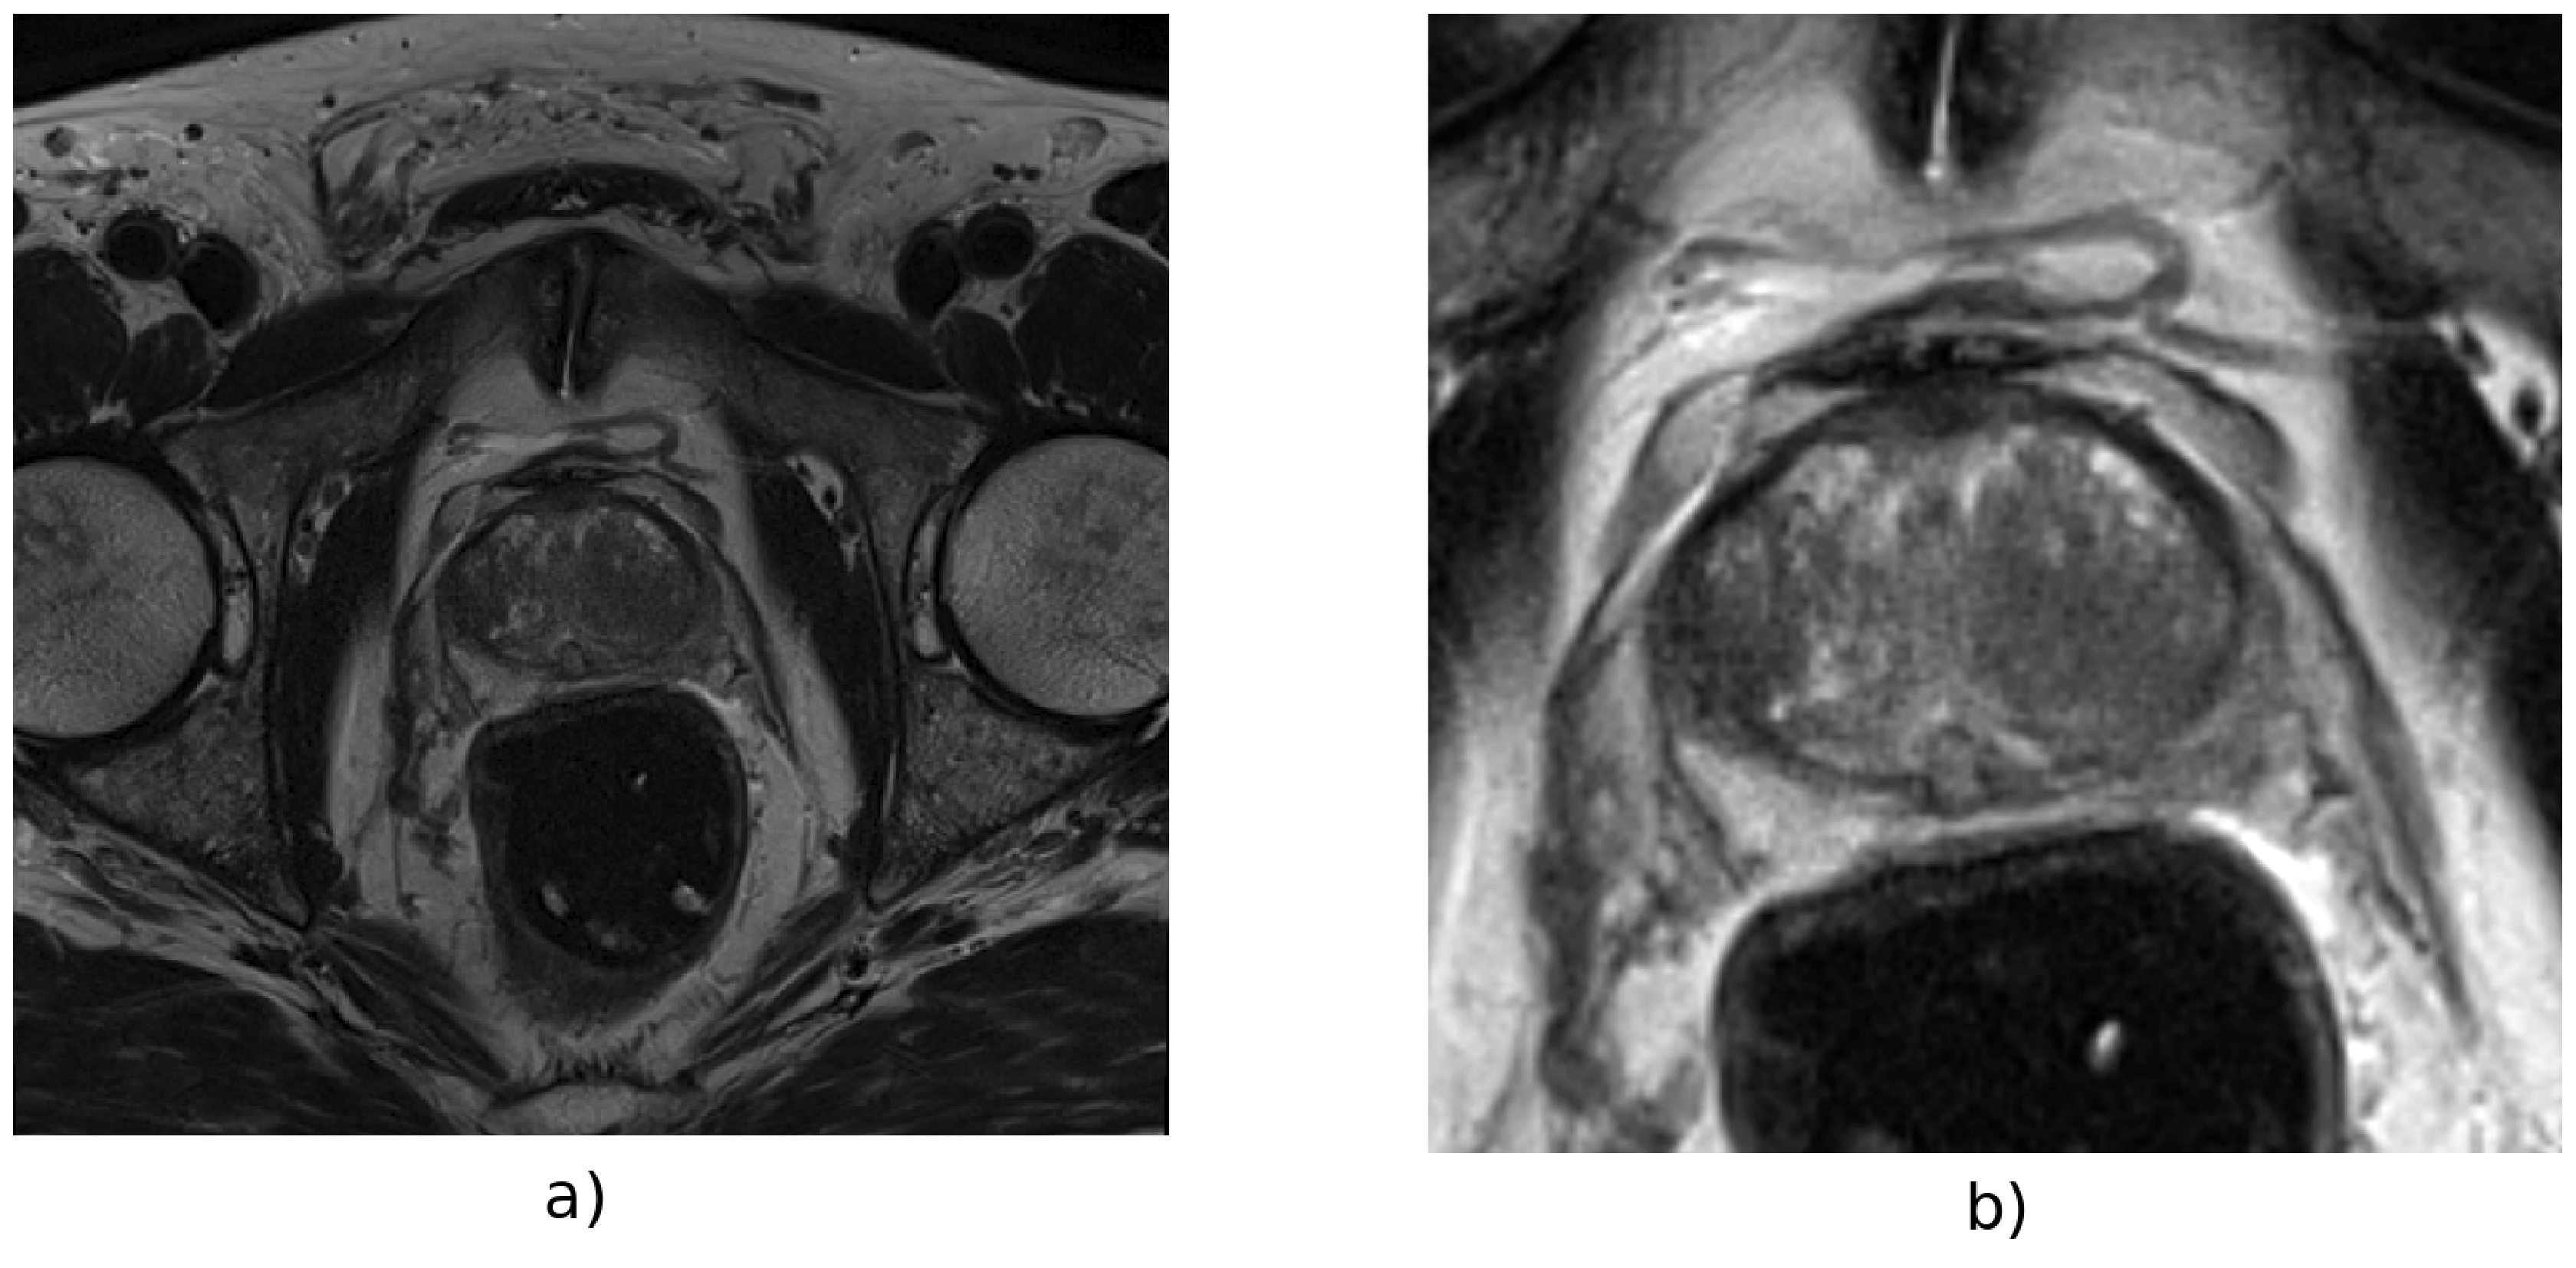
\includegraphics[totalheight=.25\textheight]{figures/Figure1.eps}
    \caption{The MRIs are preprocessed with bias correction, normalization, resampling, and cropped to a ROI to reduce the variability of sizes and intensities between magnets. In this example, \textbf{a)} is the original image and \textbf{b)} is the image after being processed.} 
    \label{fig_1}
\end{figure}

\begin{figure}[ht]
    \centering
    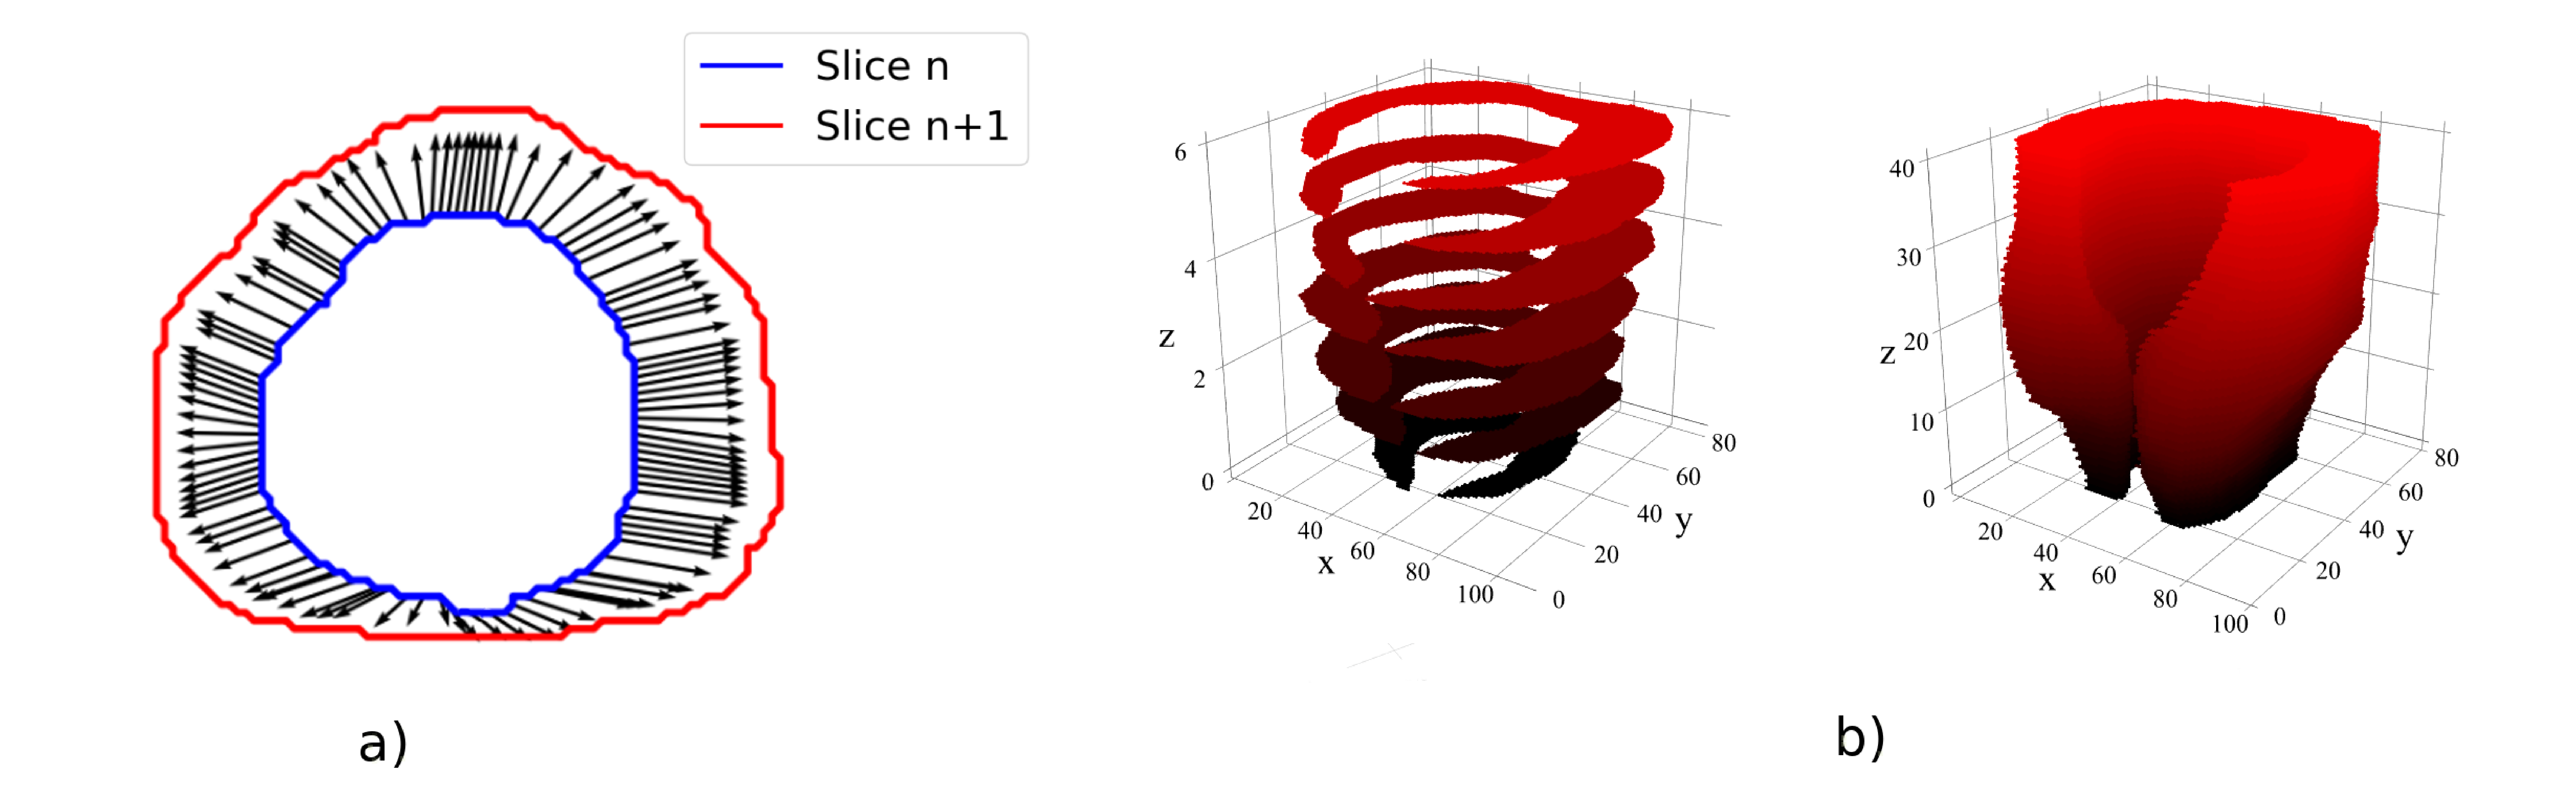
\includegraphics[totalheight=.21\textheight]{figures/Figure2.eps}
    \caption{Example of the proposed algorithm to increase the resolution of prostate and PZ contours. In \textbf{a)}, an example of the optical flow obtained between two prostate contours from adjacent horizontal planes. In \textbf{b)} on the left, original contours with 17 slices. On the right, interpolated contours with 68 slices.}
    \label{fig:fig_2}
\end{figure}

\begin{figure*}[ht]
    \centering
    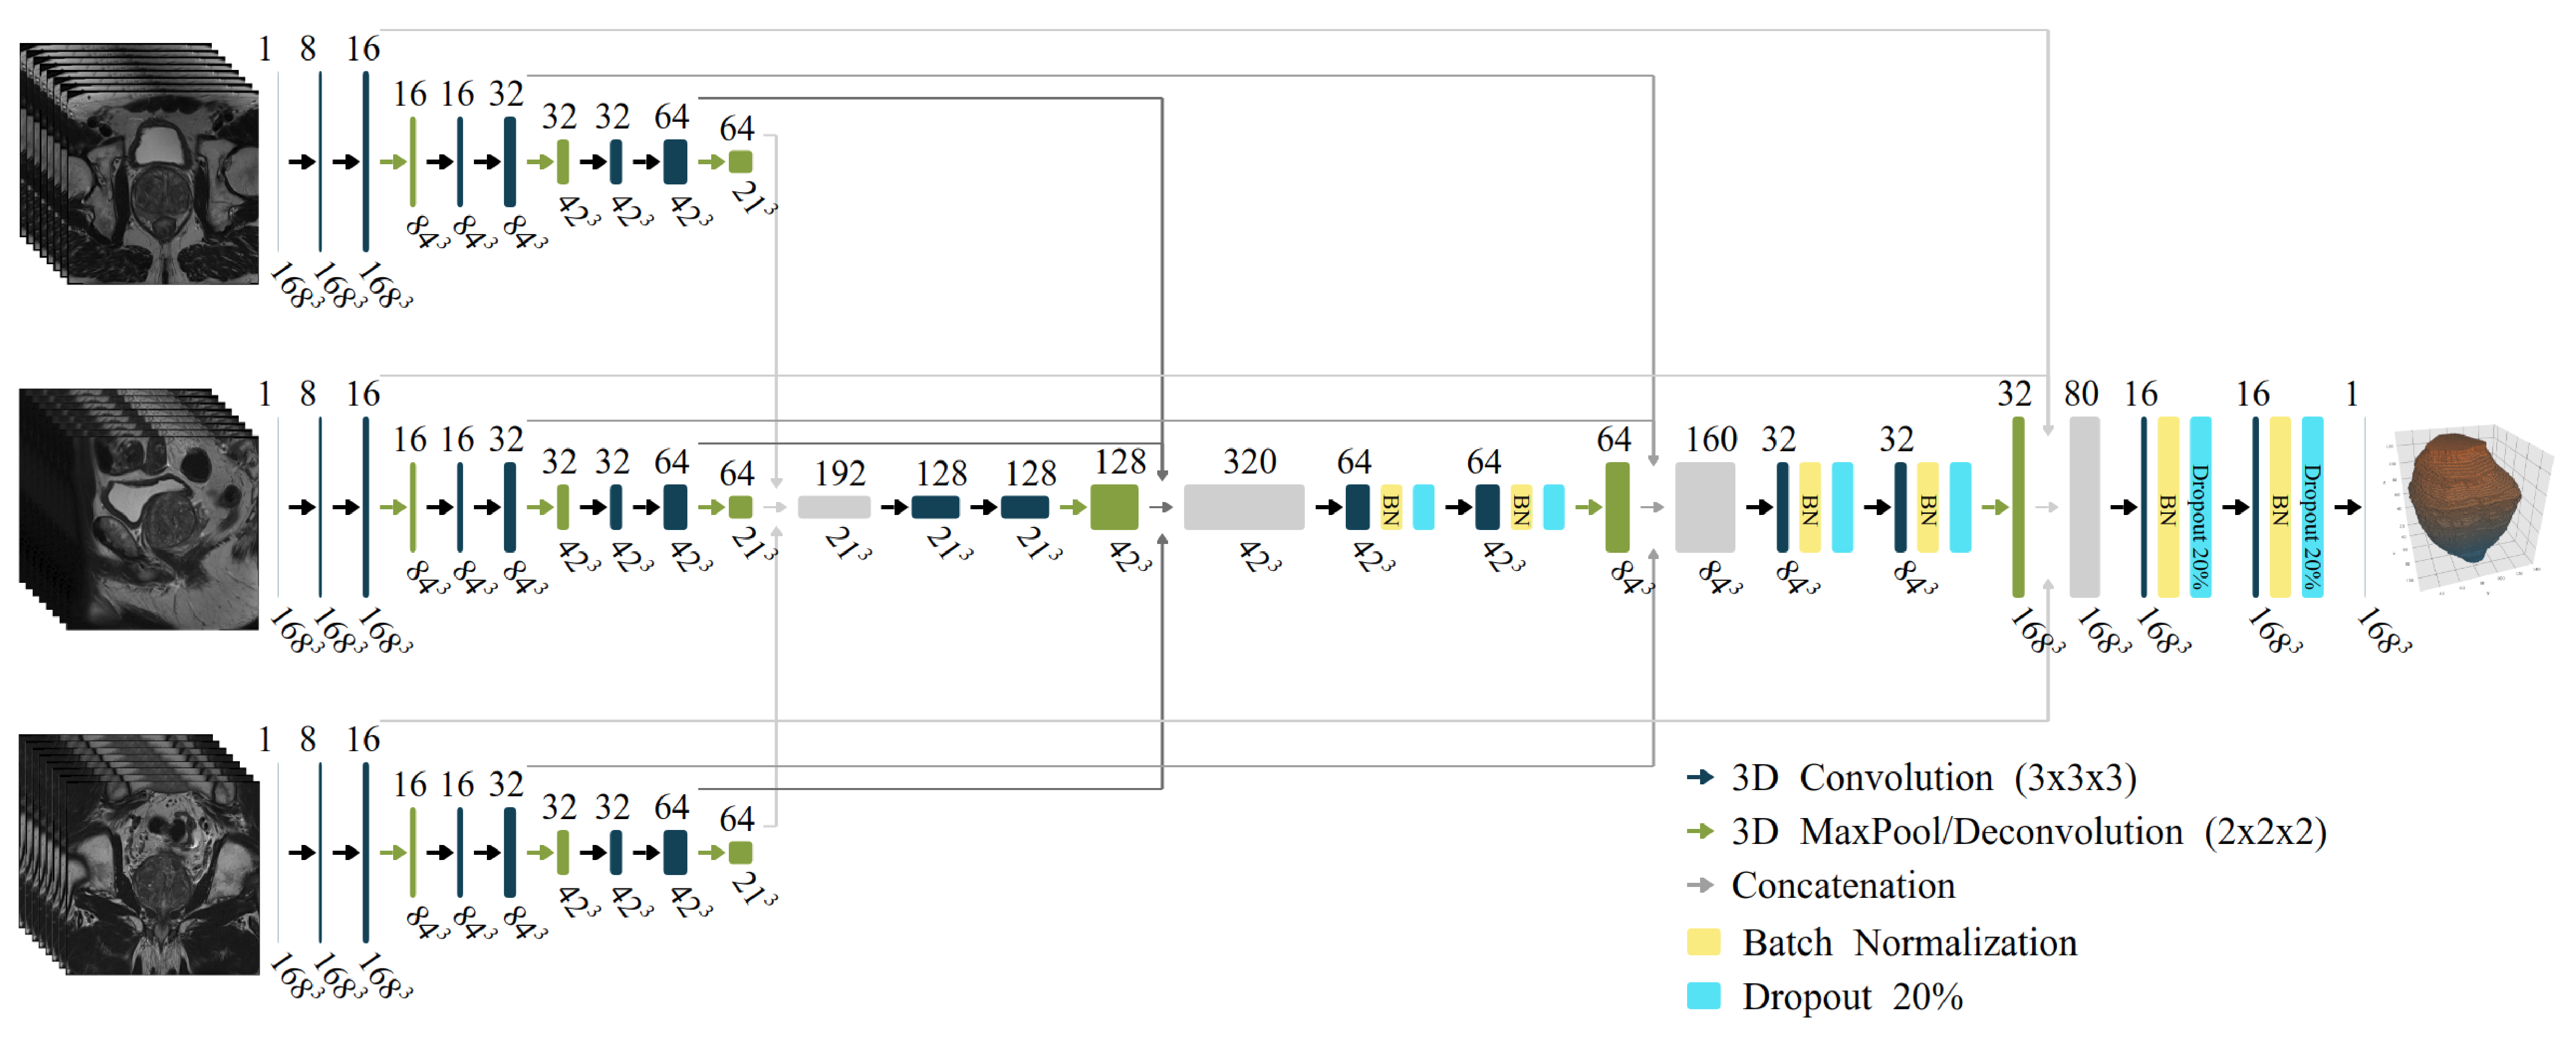
\includegraphics[totalheight=.282\textheight]{figures/Figure3.eps}
    \caption{Multistream 3D convolutional network architecture. The input of the network are three $168^3$ volumes from the MRI planes: axial, sagittal, and coronal. }
    \label{fig:fig_3}
\end{figure*}

\begin{figure}[ht]
    \centering
    \includegraphics[totalheight=.4\textheight]{figures/Figure4.eps}
    \caption{Prostate segmentation for the cases with the lowest, middle, and highest 3D DSC for the Siemens (up) and GE (down) datasets. These segmentation are obtained with the \emph{Combined} network model.  }
    \label{fig:resseg}
\end{figure} 

\begin{figure}[ht]
    \centering
    \includegraphics[totalheight=.4\textheight]{figures/Figure5.eps}
    \caption{Peripheral zone segmentation for the cases with the lowest, middle, and highest 3D DSC for the Siemens (up) and GE (down) datasets. These segmentation are obtained with the \emph{Combined} network model.  }
    \label{fig:ressegpz}
\end{figure} 



% This graphical abstract have a problem with the font
%\begin{biography}[example-image-1x1]{A.~One}
%Please check with the journal's author guidelines whether author biographies are required. They are usually only included for review-type articles, and typically require photos and brief biographies (up to 75 words) for each author.
%\bigskip
%\bigskip
%\end{biography}
% This graphical abstract have a problem with the font
%\graphicalabstract{example-image-1x1}{Please check the journal's author guildines for whether a graphical abstract, key points, new findings, or other items are required for display in the Table of Contents.}
\end{document}
